\section{Gitter}

Fælles for alle 3 systemer er kølegitteret af aluminium, der er i kontakt med processoren. 
I simple systemer udgør den den eneste part i kølesystemet og kan selvfølgelig bestå af andre materialer end Aluminium. 
Men i rapporten her vil der bliver brugt aluminum som grundlag. 

Kølegitteret udnytter overflade areal til at bortlede varme ved konvektion fra et fast materiale(aluminium) til et et fluid(atmosfærisk luft) .
Det er forfatternes påstand at kølegittere

En hyppig forekommende struktur i et kølegitter er ribbe, der giver en naturlig strømning af den varme luft bort fra kølegitteret. Hvor det kun er termodynamiske kræfter der indflyldelse på strømningen.

Der præsenteres her en oversigt over de værdier der kommer i spil i til udregningerne: 

Der beregnes varmestrøm for kovektion og for stråling.

\begin{figure}
	\centering
	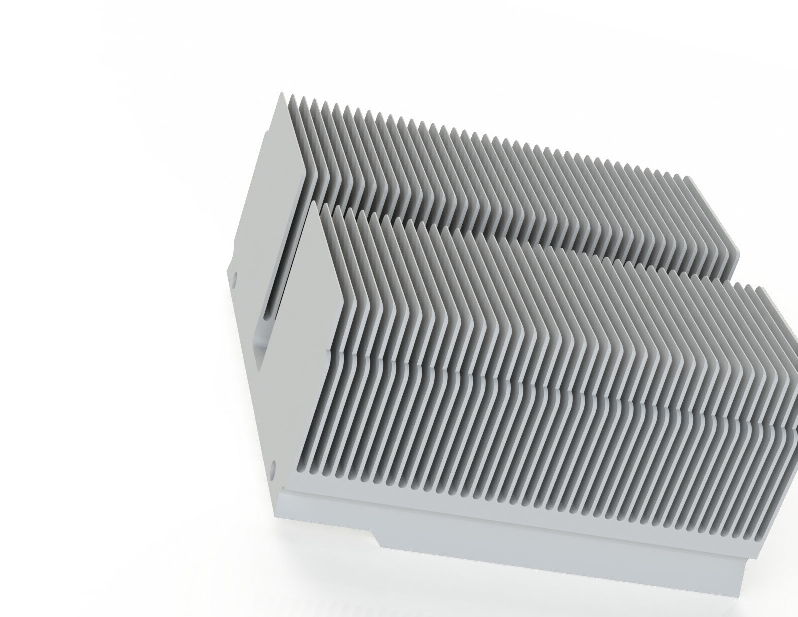
\includegraphics[width=0.7\linewidth]{billeder/heatsink1}
	\caption{Eksepel på kølegitter}
	\label{fig:heatsink1}
\end{figure}


\begin{figure}
	\centering
	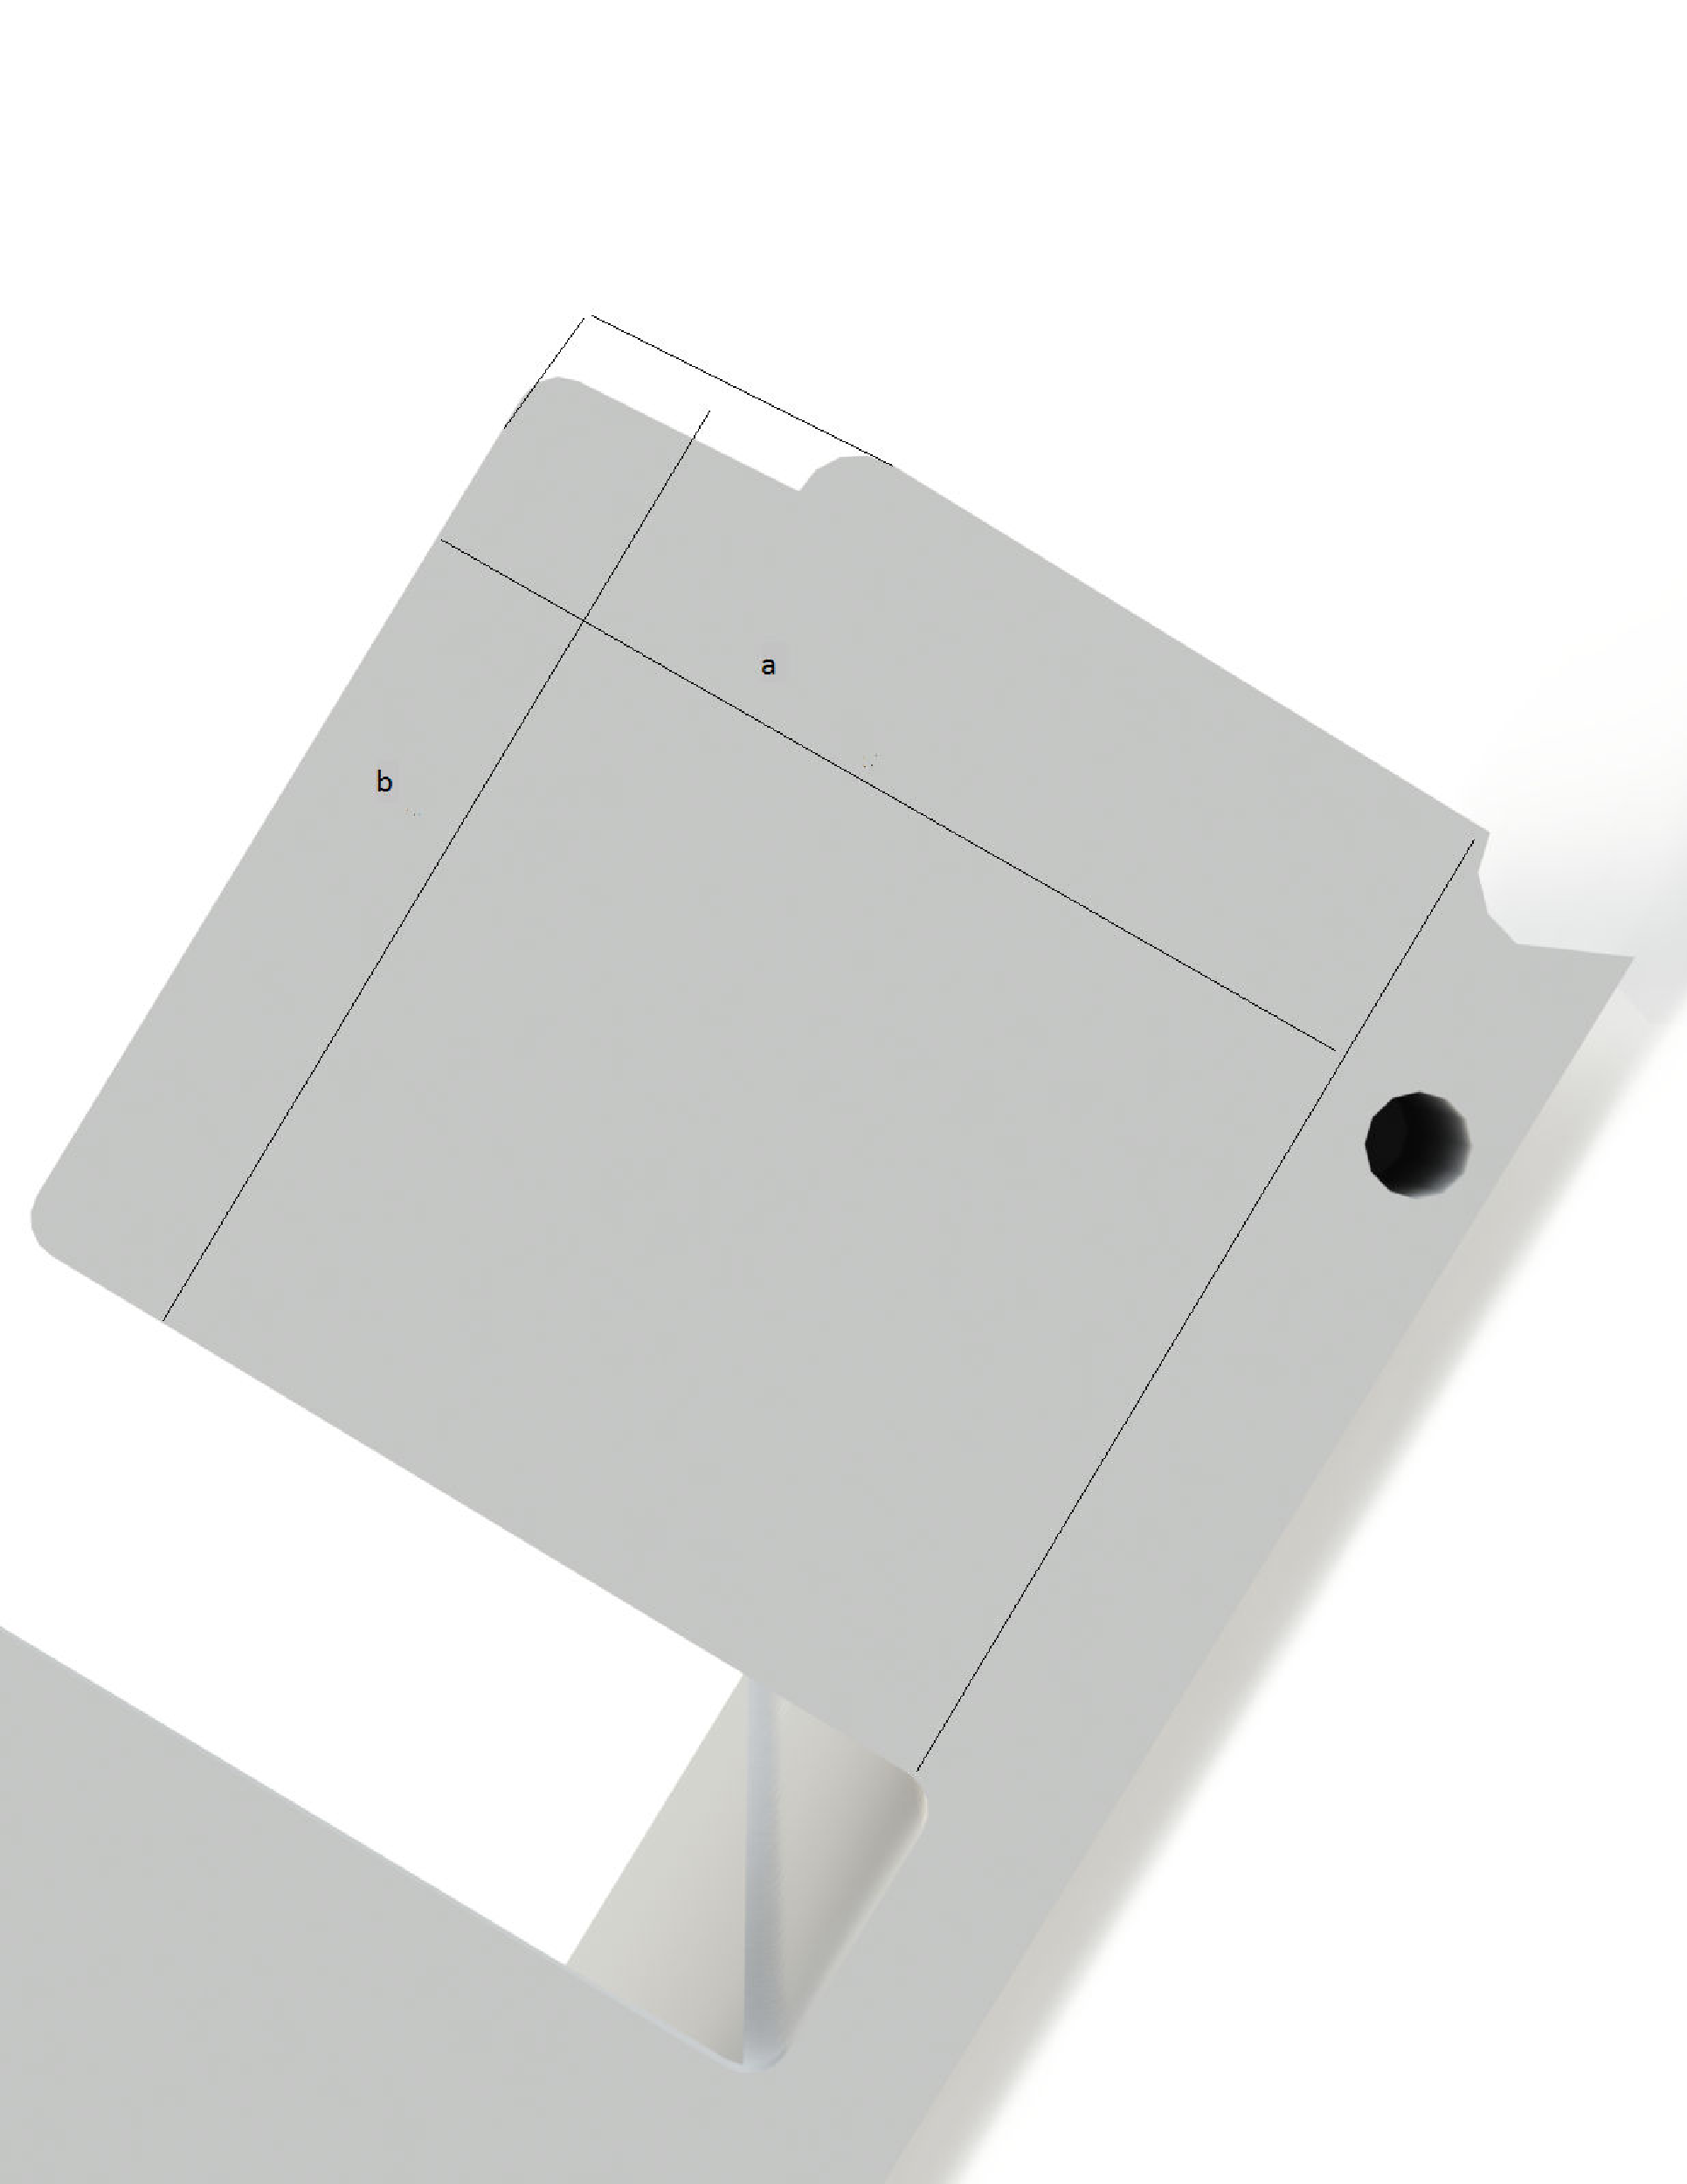
\includegraphics[width=0.7\linewidth]{billeder/lamel}
	\caption{lamel. Den mindste enhed for hvilke, vi vil undersøge de termdynamiske forhold.}
	\label{fig:lamel}
\end{figure}



Tallene for ovenstående kølegitter er importeret fra en partfil i solidworks. %Kanalen for strømningen af luft der regnes for er d(1mm) bred og den hydraulisk diameter regnes som værende en snæver kanal, hvor L=2*a

H = 20 mm, $b = 25,5 mm$, $d  =1 mm$ ,Areal $A_t = 93733.73 mm^2$ , $A_{lam}= 500 mm^2$  \\ $Massen m = 31,58 gr.$ \\
varmekonduktiviten for aluminium, $\lambda_{al} = 228$ \\  
lameltykkelsen $\delta = 0.5 mm.$  \\\
Den specifikke varmekapacitet $c\_p = 1.008$ \\
stroemningshastighed lodret, i lamellets længde på $c = 0.001$ \\



For at udregne varmestrømmen $\phi$  bruges udtrykket \\ $\Phi = \alpha * A* (t\_{fl}-t\_v$ \\  også kendt som Newtons ligning. 
Hvoraf varmekonduktiviteten $\alpha$ er fundet ved tabel opslag $\alpha = ↕21.8$
Kinematisk viskositet er: $18.88$ og dynamisk viskositet = $16.92$ 
Volumenudvidelseskoefficienten $\beta_luft = 3,2$
 


